\documentclass{beamer}
\usepackage[italian]{babel}
\usetheme{Berkeley}
\usepackage{graphicx}
\usepackage{booktabs}
% Taken from Lena Herrmann at 
% http://lenaherrmann.net/2010/05/20/javascript-syntax-highlighting-in-the-latex-listings-package
\usepackage{listings,lstautogobble,longtable}
\lstset{basicstyle=\ttfamily,breaklines=true}
\usepackage{color} %use color
\definecolor{mygreen}{rgb}{0,0.6,0}
\definecolor{mygray}{rgb}{0.5,0.5,0.5}
\definecolor{mymauve}{rgb}{0.58,0,0.82}
% Copyright 2017 Sergei Tikhomirov, MIT License
% https://github.com/s-tikhomirov/solidity-latex-highlighting/

\usepackage{listings, xcolor}

\definecolor{verylightgray}{rgb}{.97,.97,.97}

\lstdefinelanguage{Solidity}{
	keywords=[1]{anonymous, assembly, assert, balance, break, call, callcode, case, catch, class, constant, continue, constructor, contract, debugger, default, delegatecall, delete, do, else, emit, event, experimental, export, external, false, finally, for, function, gas, if, implements, import, in, indexed, instanceof, interface, internal, is, length, library, log0, log1, log2, log3, log4, memory, modifier, new, payable, pragma, private, protected, public, pure, push, require, return, returns, revert, selfdestruct, send, solidity, storage, struct, suicide, super, switch, then, this, throw, transfer, true, try, typeof, using, value, view, while, with, addmod, ecrecover, keccak256, mulmod, ripemd160, sha256, sha3}, % generic keywords including crypto operations
	keywordstyle=[1]\color{blue}\bfseries,
	keywords=[2]{address, bool, byte, bytes, bytes1, bytes2, bytes3, bytes4, bytes5, bytes6, bytes7, bytes8, bytes9, bytes10, bytes11, bytes12, bytes13, bytes14, bytes15, bytes16, bytes17, bytes18, bytes19, bytes20, bytes21, bytes22, bytes23, bytes24, bytes25, bytes26, bytes27, bytes28, bytes29, bytes30, bytes31, bytes32, enum, int, int8, int16, int24, int32, int40, int48, int56, int64, int72, int80, int88, int96, int104, int112, int120, int128, int136, int144, int152, int160, int168, int176, int184, int192, int200, int208, int216, int224, int232, int240, int248, int256, mapping, string, uint, uint8, uint16, uint24, uint32, uint40, uint48, uint56, uint64, uint72, uint80, uint88, uint96, uint104, uint112, uint120, uint128, uint136, uint144, uint152, uint160, uint168, uint176, uint184, uint192, uint200, uint208, uint216, uint224, uint232, uint240, uint248, uint256, var, void, ether, finney, szabo, wei, days, hours, minutes, seconds, weeks, years},	% types; money and time units
	keywordstyle=[2]\color{teal}\bfseries,
	keywords=[3]{block, blockhash, coinbase, difficulty, gaslimit, number, timestamp, msg, data, gas, sender, sig, value, now, tx, gasprice, origin},	% environment variables
	keywordstyle=[3]\color{violet}\bfseries,
	identifierstyle=\color{black},
	sensitive=false,
	comment=[l]{//},
	morecomment=[s]{/*}{*/},
	commentstyle=\color{gray}\ttfamily,
	stringstyle=\color{red}\ttfamily,
	morestring=[b]',
	morestring=[b]"
}

\lstset{
	language=Solidity,
	backgroundcolor=\color{verylightgray},
	extendedchars=true,
	basicstyle=\footnotesize\ttfamily,
	showstringspaces=false,
	showspaces=false,
	numbers=left,
	numberstyle=\footnotesize,
	numbersep=9pt,
	tabsize=2,
	breaklines=true,
	showtabs=false,
	captionpos=b
}

%Customize a bit the look
\lstset{ %
autogobble = true,
backgroundcolor=\color{white}, % choose the background color; you must add \usepackage{color} or \usepackage{xcolor}
basicstyle=\footnotesize, % the size of the fonts that are used for the code
breakatwhitespace=false, % sets if automatic breaks should only happen at whitespace
breaklines=true, % sets automatic line breaking
captionpos=b, % sets the caption-position to bottom
commentstyle=\color{mygreen}, % comment style
deletekeywords={...}, % if you want to delete keywords from the given language
escapeinside={<@}{@>}, % if you want to add LaTeX within your code
escapechar={|},
extendedchars=true, % lets you use non-ASCII characters; for 8-bits encodings only, does not work with UTF-8
frame=single, % adds a frame around the code
keywordstyle=\color{blue}, % keyword style
% language=Octave, % the language of the code
morekeywords={*,...}, % if you want to add more keywords to the set
numbers=left, % where to put the line-numbers; possible values are (none, left, right)
numbersep=0pt, % how far the line-numbers are from the code
numberstyle=\tiny\color{mygray}, % the style that is used for the line-numbers
rulecolor=\color{black}, % if not set, the frame-color may be changed on line-breaks within not-black text (e.g. comments (green here))
showspaces=false, % show spaces everywhere adding particular underscores; it overrides 'showstringspaces'
showstringspaces=false, % underline spaces within strings only
showtabs=false, % show tabs within strings adding particular underscores
stepnumber=1, % the step between two line-numbers. If it's 1, each line will be numbered
stringstyle=\color{mymauve}, % string literal style
tabsize=2, % sets default tabsize to 2 spaces
title=\lstname, % show the filename of files included with \lstinputlisting; also try caption instead of title
}
%END of listing package%

\definecolor{darkgray}{rgb}{.4,.4,.4}
\definecolor{purple}{rgb}{0.65, 0.12, 0.82}

%define Javascript language

\graphicspath{{figures/}}

\title{Tecniche di deep learning \\
per la classificazione di immagini biomedicali}
\author{Laureanda: Francesca Nocentini \\ Relatore: Gianluca Reali}
\institute{Università degli Studi di Perugia - Dipartimento di Ingegneria\\Corso di laurea triennale in Ingegneria Informatica ed Elettronica\\[\medskipamount]
      
\includegraphics[width=0.3\textwidth]{figures/logo_unipg.png}
 }
%\logo{\includegraphics[height=1cm]{favicon.png}}
\date{A.A. 2020/2021}

\begin{document}
\begin{frame}
	\titlepage % beamer's \maketitle
\end{frame}

\begin{frame}
	\frametitle{Indice}
	\tableofcontents
\end{frame}
\section{Premessa}

\begin{frame}
	\frametitle{AI come strumento per automatizzare l'elaborazione di grandi volumi di immagini mediche
	}
	Con l’avvento  delle  tecnologie  di imaging biomedico, il numero di immagini archiviato negli ospedali
	è divenuto di larga scala.
	
	É stato pensato dunque di sfruttare tali dati utilizzandoli
	 per allenare sistemi intelligenti che potessero assistere medici e specialisti.
	 
    \medskip
	\begin{figure}
		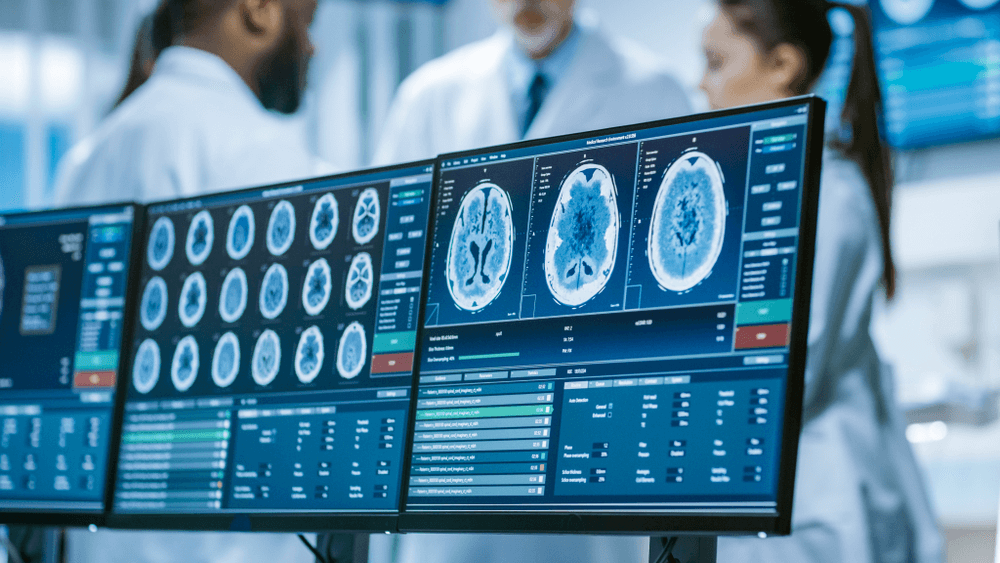
\includegraphics[width=0.65\textwidth]{imaging.png}
		% https://www.identitafutura.it/burocrazia-allitaliana/
	\end{figure}
\end{frame}


\begin{frame}
	\frametitle{L'uso delle tecniche di Deep Learning per l'apprendimento automatico
	}
	\begin{columns}
		\column{0.65\textwidth}
		\begin{figure}
			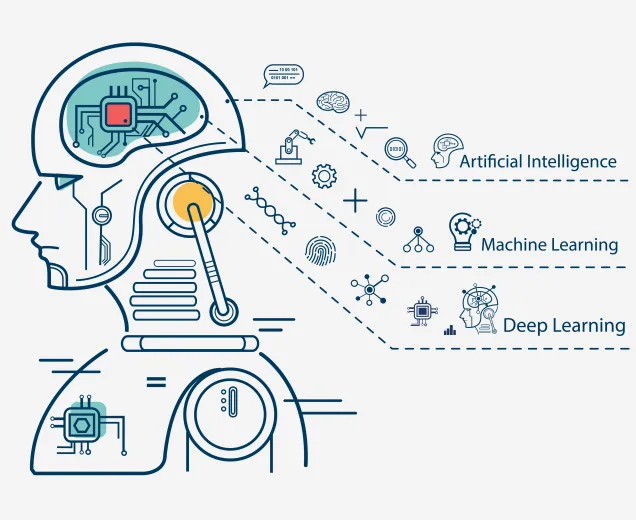
\includegraphics[width=\textwidth]{learning.png}
			% https://www.postdicom.com/it/blog/handling-dicom-medical-imaging-data
		\end{figure}
		\column{0.35\textwidth}
		Le tecniche di \textbf{Deep Learning} sono risultate essere quelle di maggior successo per la realizzazione di applicazioni per la \textbf{classificazione} di immagini mediche.
	
	In particolare è stato fatto uso di \textbf{reti neurali convoluzionali (CNN)}, sfruttando la loro architettura per l'
	\emph{image recognition}.
	\end{columns}
\end{frame}

\begin{frame}
	\frametitle{Reti neurali}
	Le \textbf{reti neurali} si riferiscono storicamente alla rete di neuroni che si trovano nel cervello 
	dei mammiferi, e la loro struttura ne ha ispirato gli algoritmi.
	%qui parlare del neurone di McCulloghs e dei pesi che vengono messi in ingresso
	% in modo tale da dare quella determinata uscita
	\medskip
	\begin{figure}
		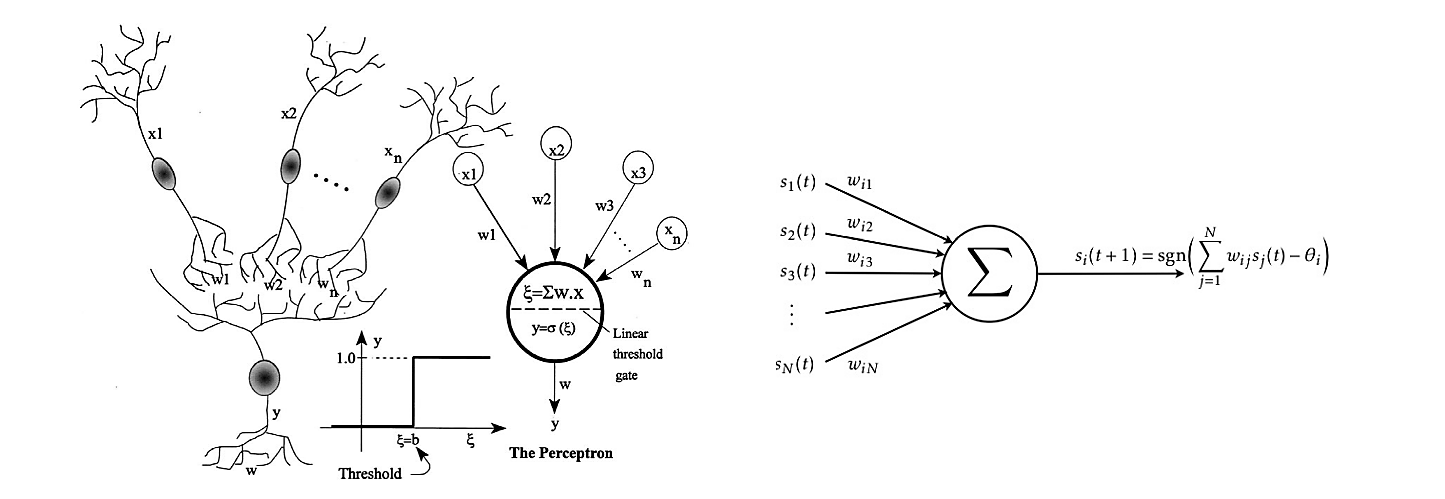
\includegraphics[width=1\textwidth]{confronto neurone biologico-artificiale.PNG}
		% https://www.identitafutura.it/burocrazia-allitaliana/
	\end{figure}
\end{frame}

\begin{frame}
	\frametitle{Le fasi dell'apprendimento della rete}
	Il punto di partenza per  addestrare  una  rete  neurale è avere a disposizione un dataset 
	formato da un insieme di \textbf{training} che viene somministrato in input alla rete per estrarne le \textbf{features},
	 e un insieme di \textbf{test} con dati completamente nuovi al sistema per verificare 
	 la sua capacità di \textbf{generalizzazione}.
	
	 \begin{figure}
		 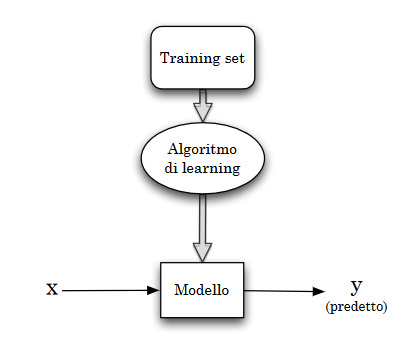
\includegraphics[width=0.65\textwidth]{schema apprendimento supervisionato.PNG}
		 
	 \end{figure}	
	
\end{frame}



\begin{frame}
	\frametitle{ }
	
	\begin{columns}
		\column{0.55\textwidth}
		\begin{figure}
			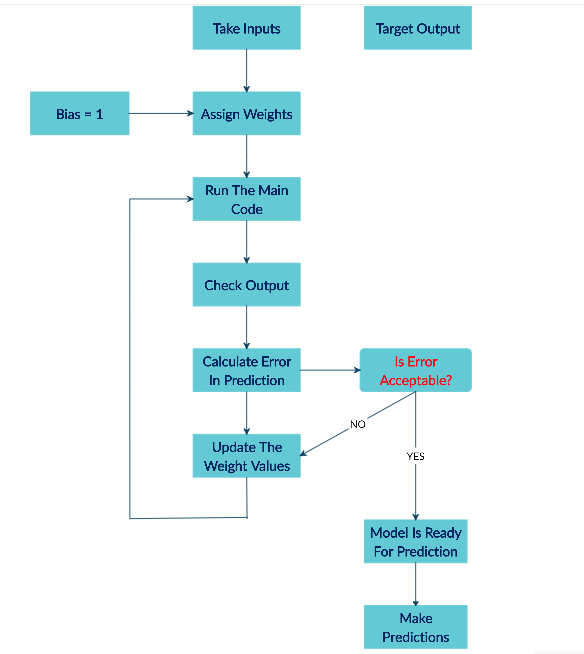
\includegraphics[width=\textwidth]{ann-flow-chart.png}
			% https://www.postdicom.com/it/blog/handling-dicom-medical-imaging-data
		\end{figure}
		\column{0.45\textwidth}
		In generale un algoritmo di apprendimento feed-forward consta di 2 fasi: 
\begin{enumerate}
   \item FEED-FORWARD 
   \item BACK-PROPAGATION
\end{enumerate} 
	\end{columns}

	
\end{frame}

\begin{frame}
	\frametitle{}
	L'algoritmo che realizza l'apprendimento minimizzando la \textbf{funzione di errore} è l'ottimizzatore.
	Esso si basa sul \textbf{Gradiente Stocastico Descrescente}, che aggiorna i pesi in questo modo: 
	\medskip
	\begin{figure}
		
\includegraphics[width=0.65\textwidth]{aggpesi.PNG}
		
	\end{figure}
	
	 %Lo scopo degli algoritmi utilizzati in questa esperienza è quello di sistemare i pesi della rete
	 % in modo da minimizzare tale funzione. 
	
\end{frame}



\begin{frame}
	\frametitle{Reti neurali convoluzionali: lo "stato dell'arte" nel riconoscimento di immagini}
	Le  Convolutional  Neural  Networks,  o  reti  di  convoluzione,  sono  reti  
	specializzate nell’elaborazione di dati che hanno la forma di vettori multipli 
	con una topologia nota a forma di griglia. 
	Esse si basano su due concetti:
	\begin{enumerate}
		\item \textbf{parameter sharing}
		\item \textbf{sparse connectivity}
	\end{enumerate}
	
	\medskip
	\begin{figure}
		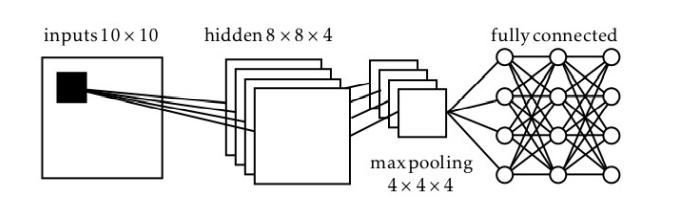
\includegraphics[width=0.65\textwidth]{cnn.PNG}
		
	\end{figure}
	
	 %Lo scopo degli algoritmi utilizzati in questa esperienza è quello di sistemare i pesi della rete
	 % in modo da minimizzare tale funzione. 
	
\end{frame}

\begin{frame}
	\frametitle{Ambiente di lavoro}
	\begin{columns}
		\column{0.3\textwidth}
		Per l’implementazione e la sperimentazione delle tecniche e dei modelli 
		di deep-learning il
		linguaggio scelto è stato Python.
		\column{0.25\textwidth}
		\centering
		\begin{figure}
			
\includegraphics[width=0.8\textwidth]{figures/python.PNG}
		\end{figure}
		\begin{figure}
			
\includegraphics[width=0.8\textwidth]{figures/index.PNG}
		\end{figure} 
		\bigskip
		\column{0.25\textwidth}
		\centering
		\bigskip\bigskip\bigskip
		\begin{figure}
			
\includegraphics[width=0.8\textwidth]{figures/scikit.PNG}
		\end{figure}
		\bigskip\bigskip
		\begin{figure}
			
\includegraphics[width=0.8\textwidth]{figures/matplotlib.JPG}
		\end{figure} 
		\column{0.20\textwidth}
		\centering
		\bigskip\bigskip\bigskip
		\begin{figure}
			
\includegraphics[width=0.7\textwidth]{figures/pandas.PNG}
		\end{figure}
		\bigskip\bigskip
		\begin{figure}
			
\includegraphics[width=0.7\textwidth]{figures/opncv.PNG}
		\end{figure} 
	\end{columns}
	
\end{frame}

\begin{frame}
	\frametitle{}
	Le librerie che sono state caratterizzanti l’esperienza di lavoro con le reti neurali sono state
TensorFlow e Keras.
\begin{figure}
	
\includegraphics[width=0.35\textwidth]{keras-tf.jpg}
	
\end{figure}
Il codice che è stato sviluppato per creare il sistema di deep learning è stato fatto girare su Jupyter e Google Collab.
\begin{figure}
	
\includegraphics[width=0.35\textwidth]{jupyter e collab.png}
	
\end{figure}

	
\end{frame}

\section{L'obiettivo}
\begin{frame}
	\frametitle{Realizzazione del sistema di classificazione}
	L’obiettivo del lavoro svolto e stato quello di utilizzare dei Dataset di immagini
	biomedicali per allenare una rete neurale convoluzionale il cui scopo è la
	classificazione delle patologie di interesse.
	L'esperienza può essere suddivisa in 2 parti:
	\begin{enumerate}
		\item classificazione di raggi-X per la rilevazione della \textbf{polmonite};
		\item uso di RM per la classificazione multipla di \textbf{tumori all'encefalo}.
	\end{enumerate}
	\begin{figure}
		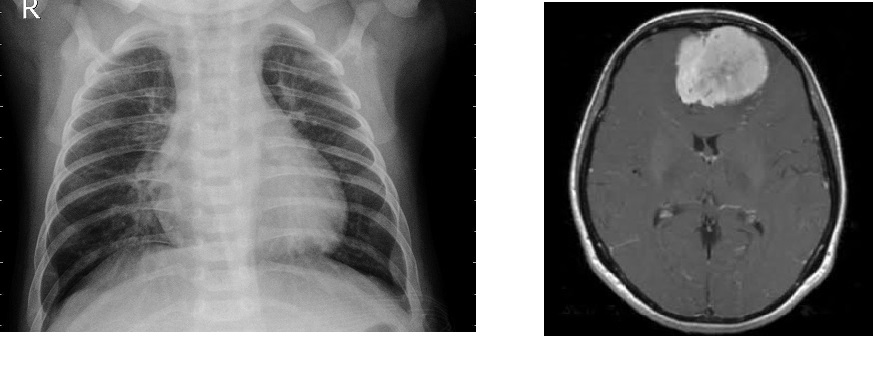
\includegraphics[width=0.65\textwidth]{virus.JPEG}
		
	\end{figure}


	 %Lo scopo degli algoritmi utilizzati in questa esperienza è quello di sistemare i pesi della rete
	 % in modo da minimizzare tale funzione. 
	
\end{frame}
\section{Rilevazione della polmonite su radiografie}
\begin{frame}
	\frametitle{Il dataset}
	Il dataset utilizzato è tratto
	 da uno studio di coorte di pazienti pediatrici di età che va da 1 a 5 anni di un centro medico di Canton (Hong Kong).
	 \smallskip
	\begin{figure}
		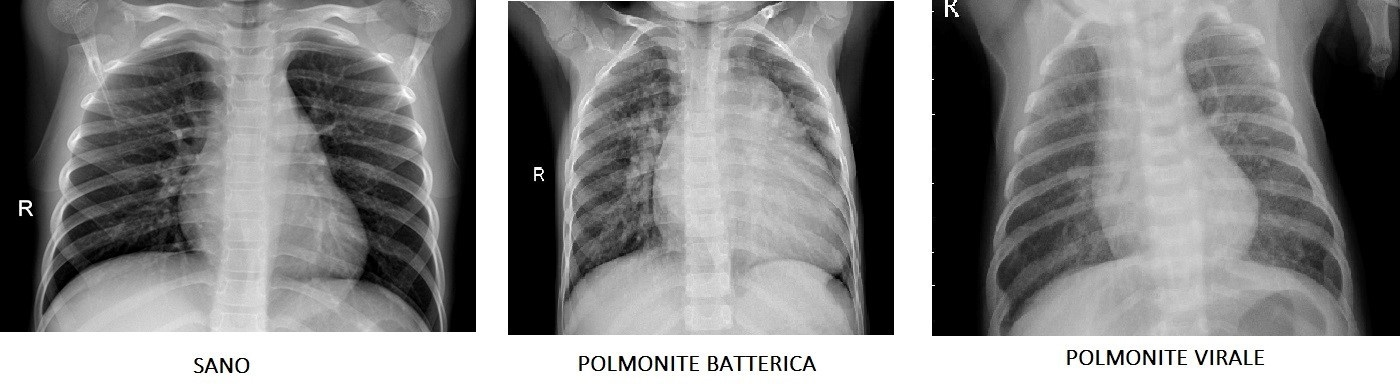
\includegraphics[width=1\textwidth]{sano.jpeg}
	\end{figure}
	Il dataset è organizzato in  3 cartelle: 
	\begin{enumerate}
		\item \textbf{Training}: 4192 immagini (1082 casi sani, 3110 di polmonite);
		\item \textbf{Testing}: 1040 immagini (267 casi sani, 773 di polmonite);
		\item \textbf{Validation}: 624 immagini (234 casi sani, 390 di polmonite).
	\end{enumerate}
	
\end{frame}

\begin{frame}
	\frametitle{Overfitting e underfitting}
	
	\begin{figure}
		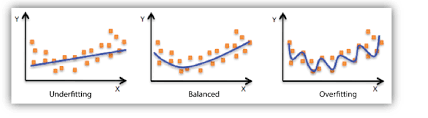
\includegraphics[width=0.7\textwidth]{ofuf.png}
	\end{figure}

		
	\begin{figure}
		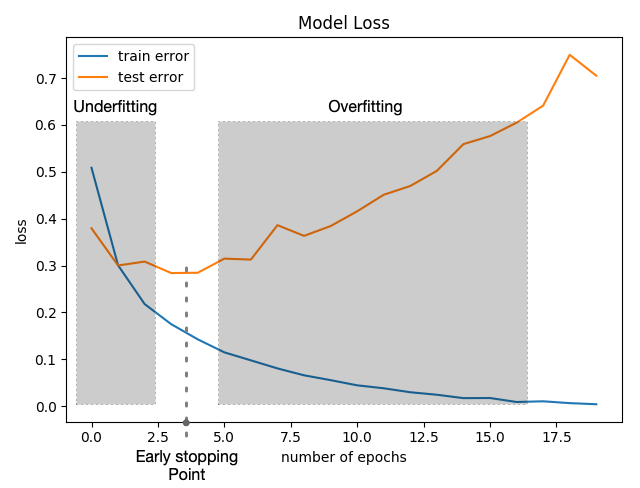
\includegraphics[width=0.7\textwidth]{ofufkeras.png}
	\end{figure}

\end{frame}

\begin{frame}
	\frametitle{Setup iniziale e definizione degli iperparametri}
	Dopo aver importato le librerie necessarie sono stati definiti dei valori per gli \textbf{iperparametri}. 
	I valori che hanno portato ad ottenere le migliori prestazioni in questa esperienza sono:
	\begin{enumerate}
		\item \lstinline[language = Python]{image_height} pari a \textbf{600};
		\item \lstinline[language = Python]{image_width} pari a \textbf{600};
		\item \lstinline[language = Python]{epochs} pari a \textbf{20};
		\item \lstinline[language = Python]{batch_size} pari a \textbf{8};
		\item \lstinline[language = Python]{hyper_featuremaps} pari a \textbf{32};
		\item \lstinline[language = Python]{hyper_channels} pari a \textbf{1}.
	\end{enumerate}

	
\end{frame}



\begin{frame}
	\frametitle{Definizione e compilazione del modello}
	Per questa esperienza è stato utilizzato un modello di rete neurale convoluzionale 
    semplice, con i seguenti strati:
	\begin{itemize}
		\item \textbf{5} strati di \textbf{Convoluzione/pooling}
		\item Strato di \textbf{flattening}
		\item \textbf{3} strati \textbf{Fully connected} rispettivamente di \textbf{128}, \textbf{64} e \textbf{1} neuroni.
	\end{itemize}

	\begin{figure}
		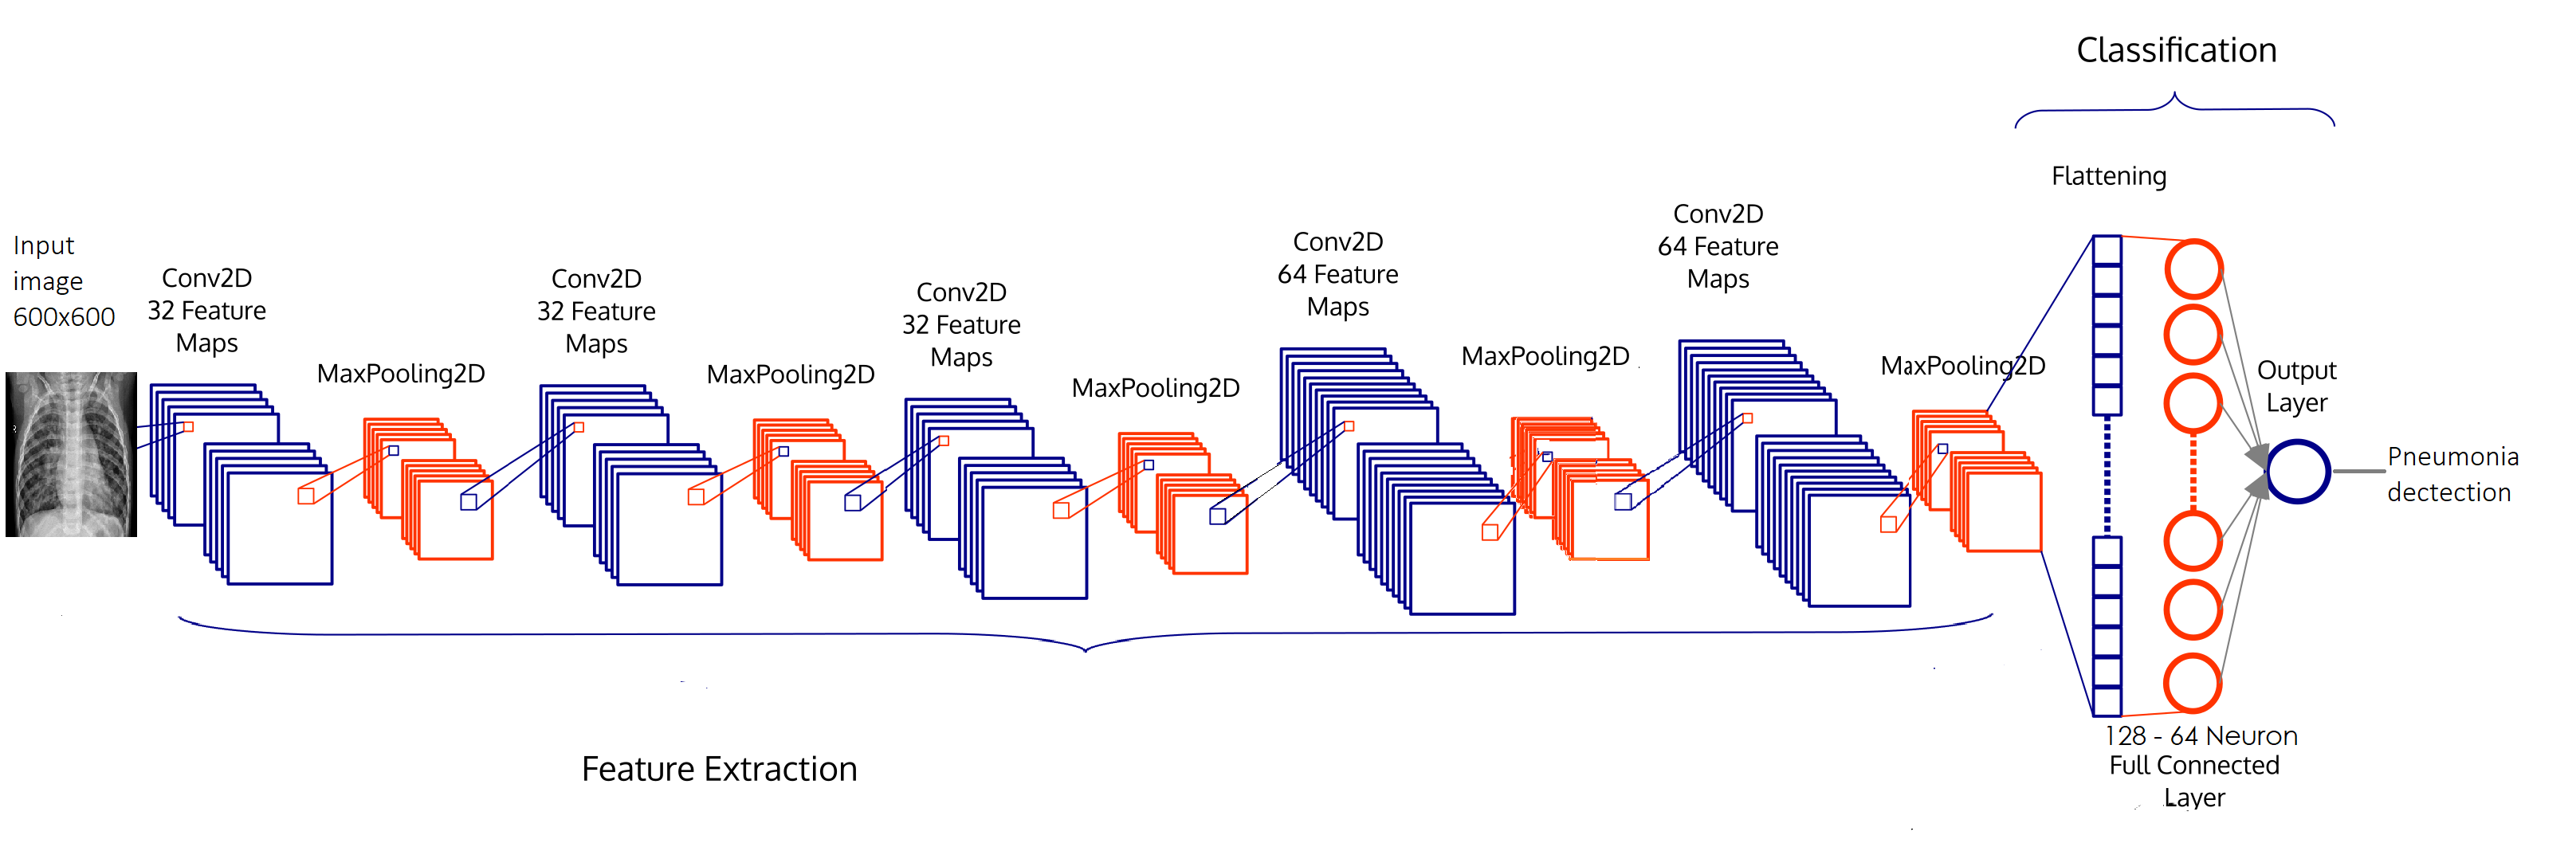
\includegraphics[width=1\textwidth]{pneumonia model.png}
	\end{figure}
		
	
\end{frame}


\begin{frame}
	\frametitle{Convoluzione2D}
	%Look at this input. We will encase the window elements with a small window,
	% dot multiplies it with the filter elements, and save the output. 
	%We will repeat each operation to derive 5 output elements as [0,0,0,1,0]. From 
	%this output, we can know that the feature change(1 becomes 0) in sequence 4.
	% The filter has done well to identify the input values. Similarly, this happened 
	%for 2D Convolutions as well.
	La convoluzione è l'operazione che consente l'estrazione delle \emph{feature} vere e proprie dall'immagine. \\
	Questa genera le \textbf{feature maps}, utilizzando dei \textbf{filtri}, (o \textbf{kernel}). 
	L'operazione compiuta è \textbf{convoluzione discreta} tra i valori dei pixel di input \textbf{I}
	e i valori dei pesi dei filtri \textbf{K}.


	%With this computation, you detect a particular feature from the input image and 
	%produce feature maps (convolved features) which emphasizes the important features. 
	%These convolved features will always change depending on the filter values affected
	% by the gradient descent to minimize prediction loss.

	%Furthermore, The more filters deployed, the more features that CNN will extract. 
	%This allows more features found but with the cost of more training time.
	% There is a sweet spot for the number of layers, usually, I will put 6 for 150 x 150 size
	% of image.
	\begin{figure}
		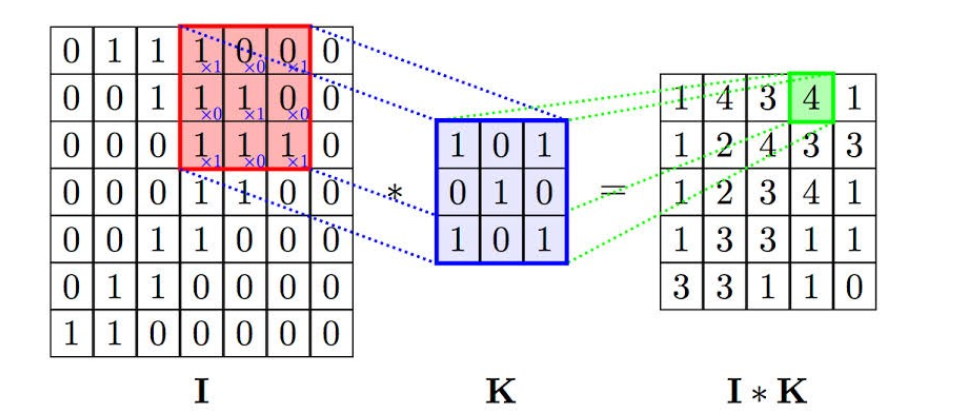
\includegraphics[width=1\textwidth]{convoluzione.PNG}
	\end{figure}
		
	
\end{frame}


\begin{frame}
	\frametitle{Pooling2D}
	Il ruolo dello strato di pooling è quello di fondere
 semanticamente feature simili in uno solo riducendo la dimensione dei dati.
 In questa esperienza è stato utilizzato il \textbf{Max-Pooling}.
	\begin{figure}
		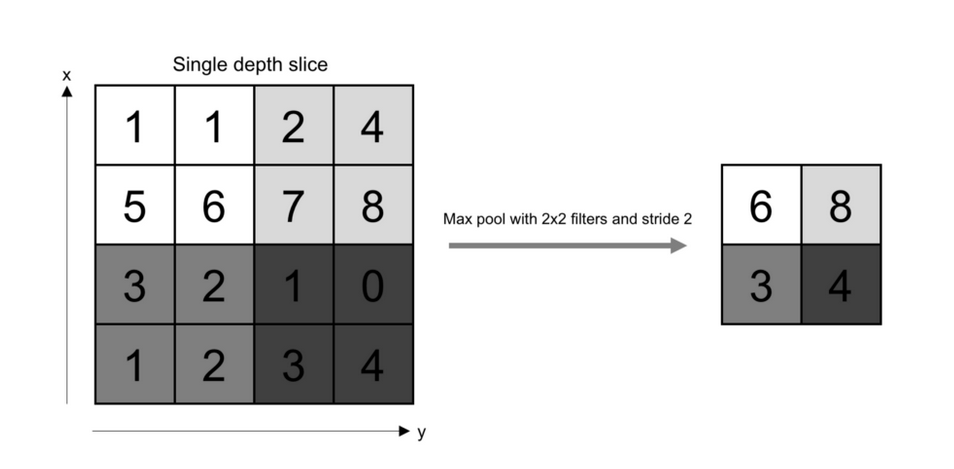
\includegraphics[width=1\textwidth]{pooling-ex.PNG}
	\end{figure}
		
	
\end{frame}



\begin{frame}
	\frametitle{Funzioni di attivazione e padding}
	É necessario che, generate le feature maps, i 
neuroni vengano passati attraverso una \textbf{funzione di attivazione}. 
Quella più utilizzata negli strati nascosti dei modelli nelle prove sperimentali è la \textbf{ReLu}
 (Rectified Linear Unit).
	\begin{figure}
		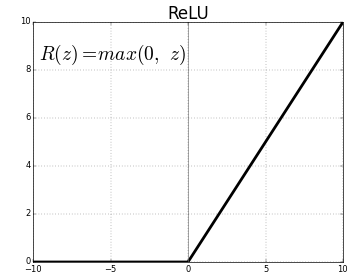
\includegraphics[width=0.3\textwidth]{relu.png}
	\end{figure}
Il tipo di padding utilizzato in questo caso è il \textbf{same padding}.
\begin{figure}
	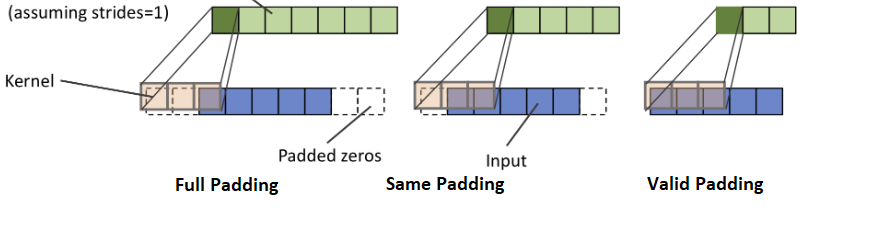
\includegraphics[width=0.6\textwidth]{padding.PNG}
\end{figure}
%Questa imbottitura aggiunge dello spazio extra attorno all'immagine che aiuta il kernel 
%a migliorare le prestazioni. Ciò è più utile se utilizzato per rilevare i bordi di un'immagine.

%Quando l'immagine sta subendo il processo di convoluzione, il kernel viene passato secondo il
% passo. Durante lo spostamento, il kernel esegue la scansione di ogni pixel e in questo
% processo esegue la scansione di pochi pixel più volte e di pochi pixel in meno (bordi).
% In generale, i pixel al centro vengono utilizzati più spesso dei pixel sugli angoli e sui bordi. 
%Ciò a sua volta può causare una scarsa rilevazione dei bordi. Possiamo superare questo problema
% usando il padding.
	
\end{frame}



\begin{frame}[fragile]
	\frametitle{Definizione e compilazione del modello tramite le classi Keras}

\begin{lstlisting}[basicstyle=\tiny, language=Python, numbers = none]
	cnn = Sequential()
	cnn.add(Conv2D(hyper_featuremaps, (3, 3), activation="relu", input_shape=(img_width, img_height, hyper_channels)))
	cnn.add(MaxPooling2D(pool_size = (2, 2)))
	...
	cnn.add(Conv2D(hyper_featuremaps * 2, (3, 3), activation="relu", input_shape=(img_width, img_height, hyper_channels)))
	cnn.add(MaxPooling2D(pool_size = (2, 2)))
	...
	cnn.add(Flatten())
	cnn.add(Dense(activation = 'relu', units = 128))
	cnn.add(Dense(activation = 'relu', units = 64))
	cnn.add(Dense(activation = 'sigmoid', units = 1))
	cnn.compile(optimizer = 'adam', loss = 'binary_crossentropy', metrics = ['accuracy'])
\end{lstlisting}
\end{frame}


\begin{frame}[fragile]
	\frametitle{Sommario del modello}
	
É possibile calcolare i \textbf{parametri} del modello, che ci permettono di stimare la \textbf{durata} del training 
e la \textbf{complessità} del modello.
\begin{lstlisting}[basicstyle=\tiny, numbers = none]
Layer (type)                 Output Shape              Param #   
=================================================================
conv2d (Conv2D)              (None, 598, 598, 32)      320       
_________________________________________________________________
max_pooling2d (MaxPooling2D) (None, 299, 299, 32)      0         
_________________________________________________________________
conv2d_1 (Conv2D)            (None, 297, 297, 32)      9248      
_________________________________________________________________
max_pooling2d_1 (MaxPooling2D) (None, 148, 148, 32)      0         
_________________________________________________________________
...
Total params: 2,179,841
Trainable params: 2,179,841
Non trainable params: 0
\end{lstlisting}
Il numero di parametri per ogni strato di convoluzione si trova come:
\begin{lstlisting}[basicstyle=\tiny, numbers = none]
(input_filters x kernel_height x kernel_width + bias) x output_filters
\end{lstlisting}
\end{frame}


\begin{frame}
	\frametitle{Creazione dei set di training e validation tramite l'uso dell'\emph{image flowing}}
	È stata utilizzata la classe di TensorFlow \lstinline{ImageDataGenerator()} per fare \emph{image augmentation}.
	Le tecniche che sono risultate essere utili in questo caso sono:
	\begin{itemize}
	  \item \textbf{Rescaling}: 1./255;
	  \item \textbf{Random Rotation}: tra i -5$^\circ$  e i 5$^\circ$;
	   \item \textbf{Random Zoom}: range (100-120)$\%$ dell'immagine originale.
	   %adds some pixels around the image to enlarge the image.
	\end{itemize}
	\begin{figure}
		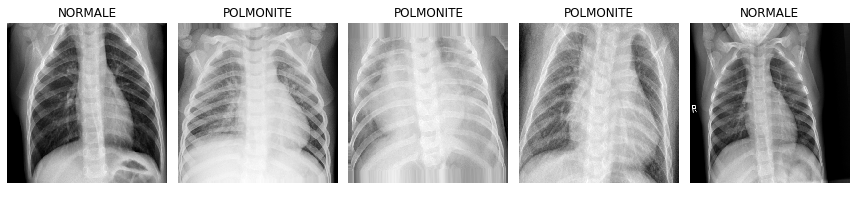
\includegraphics[width=1\textwidth]{best-augmented-images-pneumonia.png}
	\end{figure}

	
\end{frame}


\begin{frame}[fragile]
	\frametitle{Fitting del modello}
	La tupla \textbf{train = (X\_train, y\_train)} generata è stata data in pasto alla rete
	 a gruppi di immagini pari alla \lstinline[language = Python]{batch_size}.
	Tutto il dataset è stato rivisitato interamente un numero di volte pari a \lstinline[language = Python]{epochs}.
	La metrica utilizzata è l'\textbf{accuratezza}. %accuracy is the fraction of 
	%predictions our model got right
	\begin{lstlisting}[basicstyle=\tiny, language=Python, numbers = none]
		history = cnn.fit(train,epochs=20, validation_data=valid, class_weight=cw, callbacks=callbacks_list)
		
	\end{lstlisting}
Output estrapolato da uno dei training eseguiti sul set ampliato:
\smallskip
\begin{lstlisting}[basicstyle=\tiny, numbers = none]
Epoch 1/20
524/524 [==============================] - 205s 329ms/step - loss: 0.4091 - accuracy: 0.7891 - val_loss: 0.4192 - val_accuracy: 0.8183

Epoch 00001: val_accuracy improved from -inf to 0.81827

Epoch 2/20
524/524 [==============================] - 174s 332ms/step - loss: 0.2235 - accuracy: 0.9086 - val_loss: 0.2181 - val_accuracy: 0.9144

Epoch 00002: val_accuracy improved from 0.81827 to 0.91442
...
\end{lstlisting}
\end{frame}


\begin{frame}
	\frametitle{Andamento del training}
	Sono stati confrontati i training eseguiti su due set differenti:
	\begin{enumerate}
		\item il set di training originale;
		\item il set di training ampliato con le tecniche di scaling, zooming e rotating.
	\end{enumerate}

	\begin{figure}
		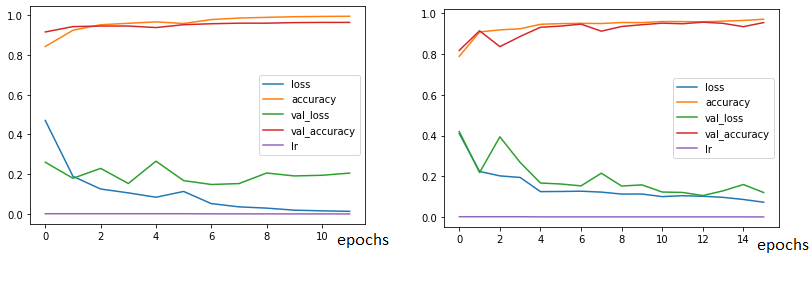
\includegraphics[width=1\textwidth]{history-pneumonia-no-aug.png}
	\end{figure}

	
\end{frame}


\begin{frame}
	\frametitle{Previsioni e risultati ottenuti}
	Sono stati ottenuti i seguenti risultati (in termini di \textbf{accuracy}):
	\begin{enumerate}
		\item sul set di training originale:

	\begin{table}[width=0.8\textwidth]
		\begin{tabular}{lll}
		\textbf{Training} & \textbf{Validation} & \textbf{Testing} \\ \hline
		(99.61 $\pm$ 0.01) \%           & (94.44  $\pm$ 0.01)\%   &	(\textbf{75.80} $\pm$ 0.01)\%         
		\end{tabular}
		\end{table}
		\smallskip

	
				\item sul set di training ampliato:
	
	\begin{table}[width=0.8\textwidth]
		\begin{tabular}{lll}
		\textbf{Training}  & \textbf{Validation} & \textbf{Testing} \\ \hline
		(96.49 $\pm$ 0.01) \%           & (94.61  $\pm$ 0.01)\%   &	(\textbf{93.75} $\pm$ 0.01)\%         
		\end{tabular}
		\end{table}
	\end{enumerate}
	
\end{frame}


\begin{frame}
	\frametitle{Matrici di confusione}
	Si mostrano le \textbf{matrici di confusione} ottenute nei due casi:
	\medskip
	\begin{figure}
		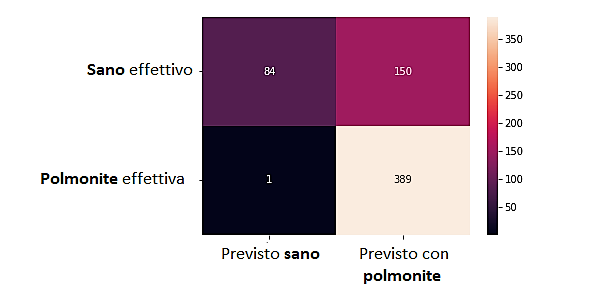
\includegraphics[width=0.7\textwidth]{conf-matrix-no-aug.png}
	\end{figure}

\begin{figure}
	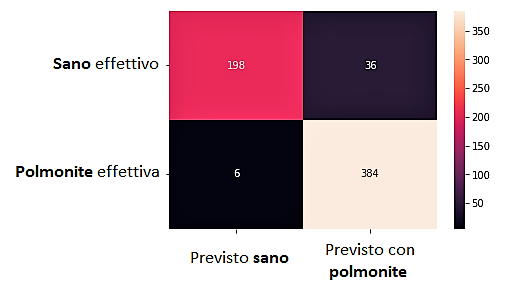
\includegraphics[width=0.6\textwidth]{conf-matrix-pneumonia-aug.png}
\end{figure}	
\end{frame}


\begin{frame}
	\frametitle{Receiver Operating Characteristic}
	Si mostrano le curve \textbf{ROC} e le relative \textbf{AUC} nei due casi:
	\begin{figure}
		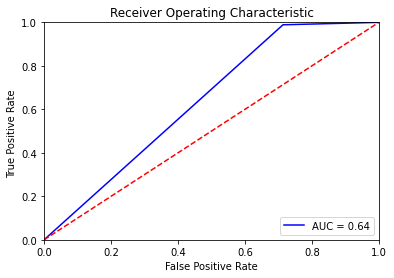
\includegraphics[width=0.5\textwidth]{roc-pneumonia-no-aug.png}
	\end{figure}

\begin{figure}
	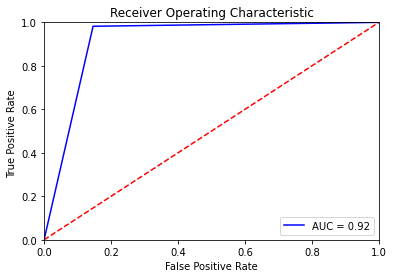
\includegraphics[width=0.5\textwidth]{roc-pneumonia-aug.png}
\end{figure}	
\end{frame}


\begin{frame}
	\frametitle{Dimostrazione su alcune immagini prese dall'insieme di test}
	
	\begin{figure}
		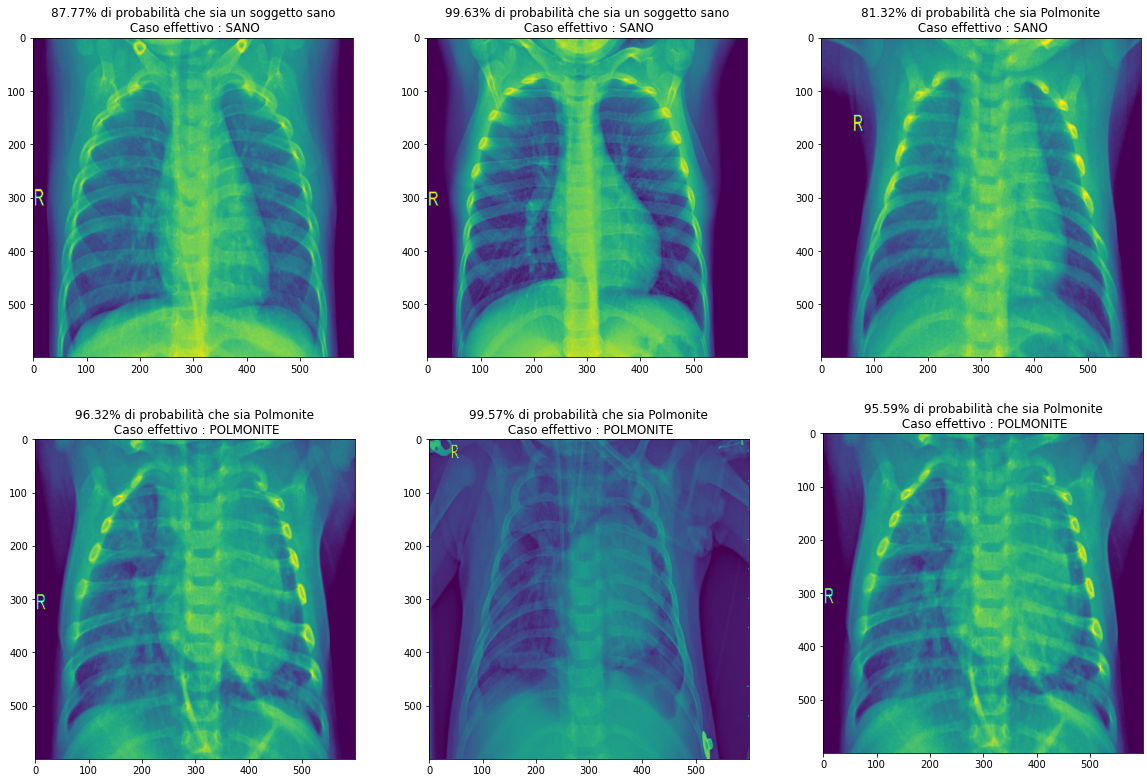
\includegraphics[width=1\textwidth]{pneumonia results.png}
	\end{figure}

\end{frame}

\begin{frame}
	\frametitle{Conclusioni}
	In sostanza ciò che ha permesso di ottenere un buon modello senza andare in underfitting
	e overfitting è stato:
	\begin{itemize}
		\item un buon dataset;
		\item l'uso dell'\textbf{image augmentation};
		\item dei buoni iperparametri;
		\item un modello semplice ma equilibrato rispetto alle dimensioni del dataset;
		\item l'uso della funzione \textbf{EarlyStopping()}.
	\end{itemize}
	
\end{frame}

\section{Classificazione di RM all'encefalo}


\begin{frame}
	\frametitle{Il Dataset}
	Nel dataset vi sono \textbf{3264} immagini che 
	riportano \textbf{RM} encefaliche raggruppate 
	 in \textbf{2} folder.
Nella \textbf{training folder} ci sono:
\begin{itemize}
	\item \textbf{395} immagini dell’encefalo \textbf{sano},
	\item \textbf{827} del tumore \textbf{ipofisario},
	\item \textbf{822} del \textbf{meningioma},
	\item \textbf{826} del \textbf{glioma}. 
\end{itemize}
Nella \textbf{testing folder} ci sono:
\begin{itemize}
	\item \textbf{105} immagini di encefalo \textbf{sano},
	\item \textbf{74} di tumore \textbf{ipofisario}, 
	\item \textbf{115} di \textbf{meningioma},
	\item \textbf{100} di \textbf{glioma}. 
\end{itemize}
\end{frame}

\begin{frame}[fragile]
Il tipo di classificazione che viene fatta in questa esperienza è \textbf{multiclasse}.
Si utilizzano le seguenti label:
\begin{lstlisting}[basicstyle=\tiny, language = Python, numbers = none]
	labels = ['glioma_tumor','meningioma_tumor','no_tumor','pituitary_tumor']
\end{lstlisting}
\begin{figure}
	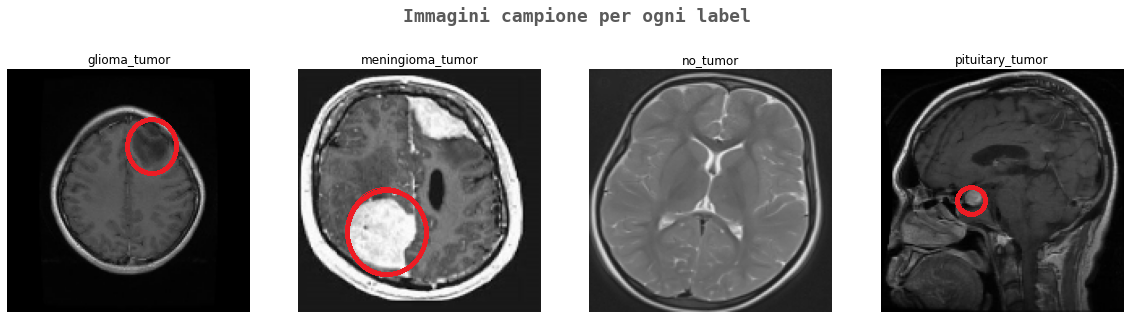
\includegraphics[width=1\textwidth]{brain-samples.png}
\end{figure}

\end{frame}


\begin{frame}
	\frametitle{Definizione degli iperparametri e dei modelli utilizzati}
	Sono stati fatti dei training su 3 modelli differenti:
	\begin{enumerate}
		\item Una CNN generica come in figura;	
	\end{enumerate}
		\begin{figure}
			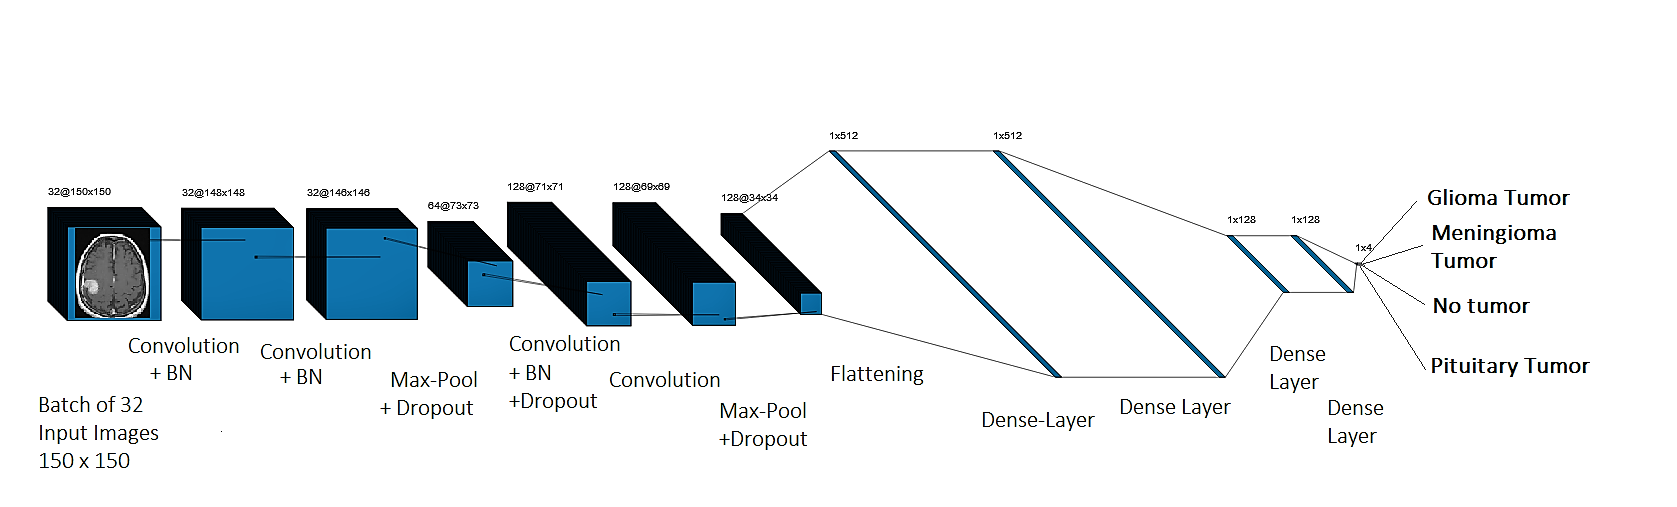
\includegraphics[width=1.1\textwidth]{BT-first.PNG}
		\end{figure}
		
	
\end{frame}



\begin{frame}
	
	\begin{enumerate}
		\setcounter{enumi}{1}
		\item \textbf{AlexNet} nella versione utilizzata nel 2012 per una competizione su un dataset di larga scala come \textbf{ImageNet}, rivisitata sulla base degli obiettivi di questa classificazione;	
	\end{enumerate}
		\begin{figure}
			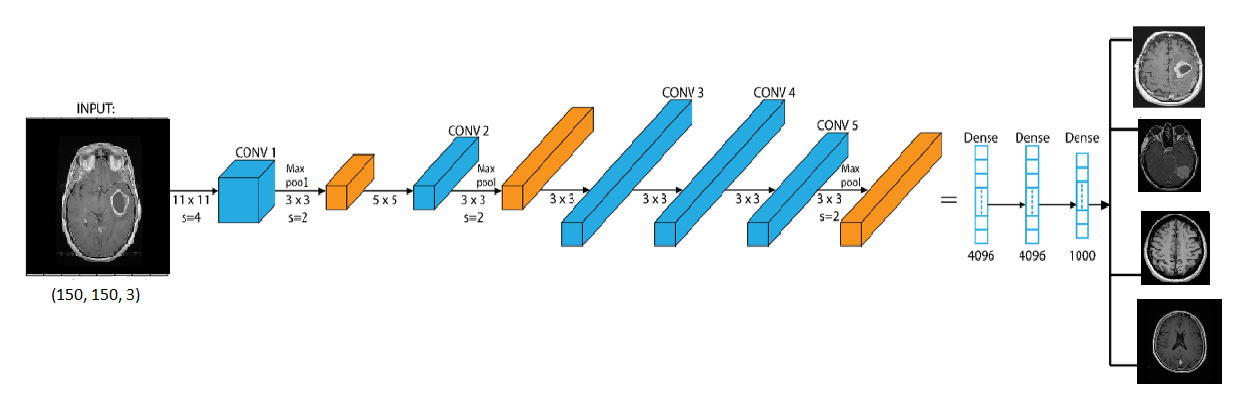
\includegraphics[width=1\textwidth]{AlexNet.PNG}
		\end{figure}
		
	
\end{frame}


	
\begin{frame}
	
	\begin{enumerate}
		\setcounter{enumi}{2}
		\item In questo ultimo caso si applica il concetto di \textbf{Transfer Learning}, utilizzando un modello precedentemente allenato per il dataset ImageNet,
		ovvero \textbf{EfficientNetB0}.\\
		Tale modello utilizza il concetto di Convoluzione2D unita ad una Convoluzione \textbf{DepthWise} andando ad abbassare il costo computazionale e la durata del training.
	\end{enumerate}
		\begin{figure}
			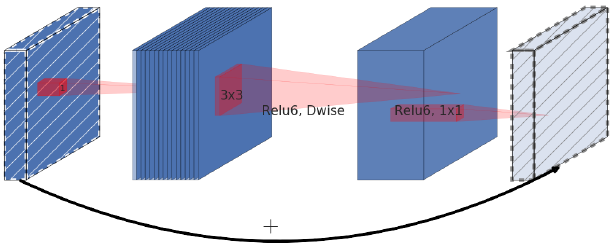
\includegraphics[width=1\textwidth]{efficientnet.png}
		\end{figure}
		
	
\end{frame}


\begin{frame}
	\frametitle{Dropout e BatchNormalization per evitare overfitting}
		Buona norma è quella di ridimensionare la rete neurale leggermente in eccesso utilizzando il \textbf{Dropout},
		che permette di evitare attivazioni nascoste che potrebbero portare a overfitting. \\
		%Di solito questo viene posizionato tra gli strati densi e così èè stato fatto con AlexNet
		\begin{figure}
			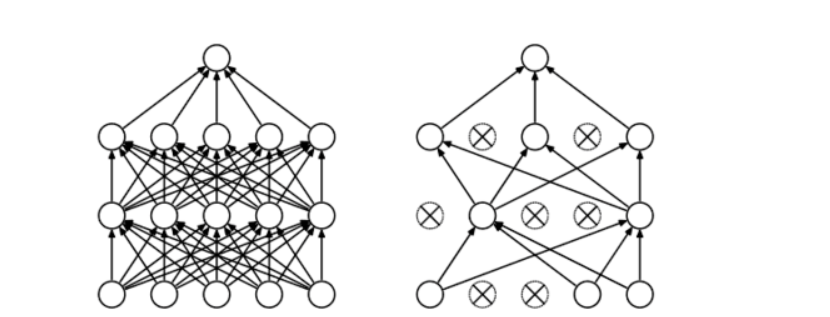
\includegraphics[width=1\textwidth]{dropout.PNG}
		\end{figure}
		Inoltre è possibile dar maggior robustezza con strati di \textbf{BatchNormalization}.
		La normalizzazione batch scala gli output dei livelli della CNN in modo che abbiano media 0 e varianza 1.\\
		% Gli output vengono ridimensionati in modo da addestrare la rete più 
		%velocemente. Riduce anche i problemi dovuti a una scarsa inizializzazione
		% dei parametri.
		%Normalizzare i dati uniforma la varianza e la dev std così che la funzione di costo da minimizzare
		%sia più simmetrica e sia possibile utilizzare un learning rate più grande così da apprendere più velocemente
		%è una tecnica di regolarizzazione così come il dropout
		%fa decrescere l'importanza di come sono stati inizializzati i pesi
		%si normalizza sottraendo il valor medio e dividendo per la std dev
	\end{frame}


\begin{frame}[fragile]
\frametitle{Creazione dei set di training e testing}
Dopo aver letto e ridimensionato tutte le immagini, queste vengono inserite nel
Numpy array \textbf{X\_train} associate alla label corrispodente in \textbf{y\_train} 
codificata in codice \textbf{one-hot}.
L'utilizzo della funzione \lstinline{train_test_split()} ha permesso di creare 
un set di testing che fosse il 10\%  di quello di training.\\
Per ogni coppia \textbf{(X\_train, y\_train)} sono stati eseguiti 5 training per ciascun modello.
\end{frame}

\begin{frame}[fragile]
	\frametitle{Iperparametri utilizzati e fase di fitting}
		Ogni training è stato eseguito con tali iperparametri:
		\begin{itemize}
			\item \lstinline[language = Python]{image_height} pari a \textbf{150}, \textbf{224};
			\item \lstinline[language = Python]{image_width} pari a \textbf{150}, \textbf{224};
			\item \lstinline[language = Python]{epochs} = \textbf{40};
			\item \lstinline[language = Python]{batch_size} = \textbf{32};
			\item \lstinline[language = Python]{hyper_channels} = \textbf{3}.
			\item Ottimizzatore Adam (learning rate iniziale pari a \textbf{0.01})
		\end{itemize}
\end{frame}

\begin{frame}
	\frametitle{Aggiunta di rumore gaussiano alle immagini}
	Applicare le tecniche geometriche di ampliamento del dataset del caso dei raggi-X non ha comportato miglioramenti.\\
	Sono state utilizzate tecniche che modificassero l'\textbf{intensità dei pixel}.
	In particolare è stato aggiunto \textbf{rumore gaussiano} al set di training,
	 il quale aiuta il sistema nella \textbf{generalizzazione}. 
	 \begin{figure}
		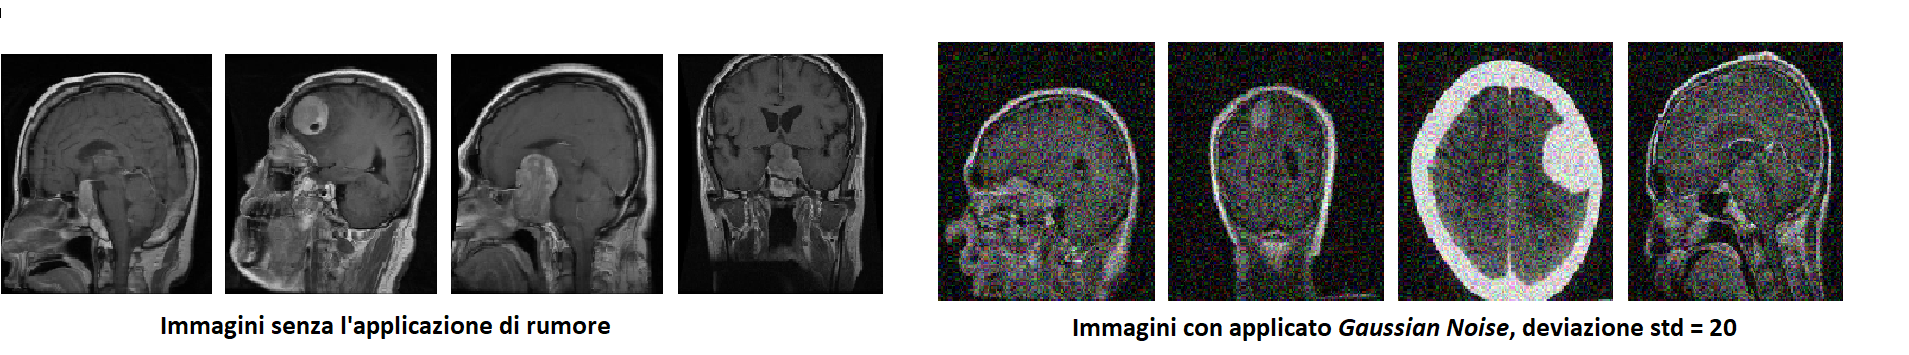
\includegraphics[width=1\textwidth]{images-noise-var-20.png}
	\end{figure}
	

	 
\end{frame}





\begin{frame}
	\frametitle{Risultati ottenuti}
			Nei 3 casi i migliori risultati ottenuti in media su 5 training per modello sono i seguenti:
			\begin{table}[]
				\begin{tabular}{lll}
													 & \textbf{Training accuracy} & \textbf{Testing accuracy} \\ \hline
				\multicolumn{1}{l|}{\textbf{Primo modello}}   & 99.2\%            & 92.2\%           \\
				\multicolumn{1}{l|}{\textbf{Secondo modello}} & 97.5\%            & 95.7\%           \\
				\multicolumn{1}{l|}{\textbf{Terzo modello}}   & 99.1\%            & 99.1\%          
				\end{tabular}
				\end{table}
	\end{frame}

	\begin{frame}
		\frametitle{Matrice di confusione: Primo modello}
		\begin{figure}
			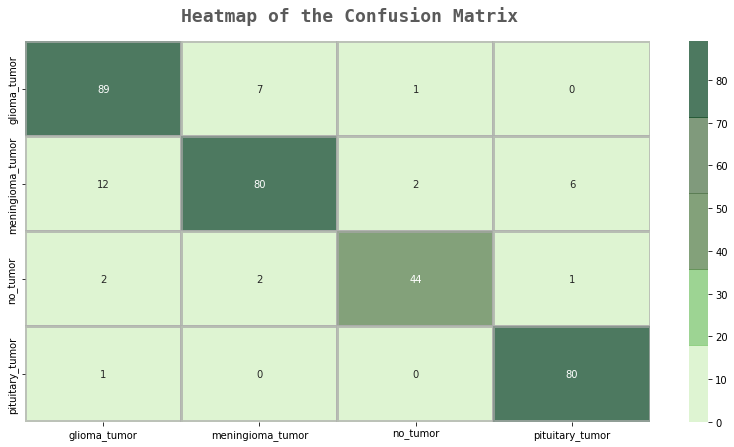
\includegraphics[width=0.9\textwidth]{conf-matrix-first.png}
		\end{figure}
	\end{frame}

\begin{frame}
	\frametitle{Matrice di confusione: Modello AlexNet con rumore}
	\begin{figure}
		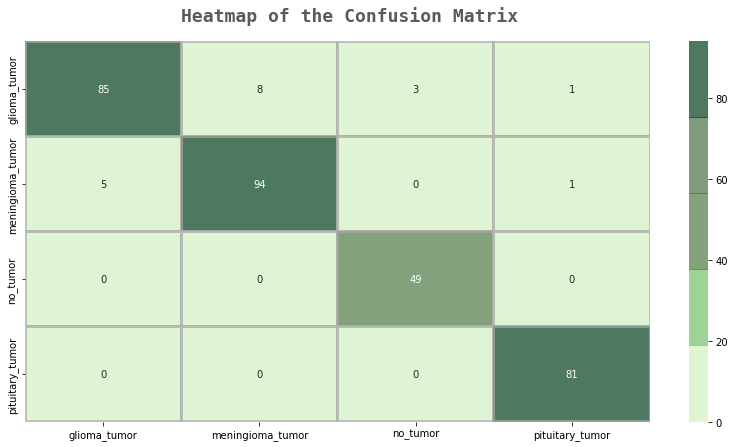
\includegraphics[width=0.9\textwidth]{conf-matrix-alex.png}
	\end{figure}
	
\end{frame}


\begin{frame}
	\frametitle{Matrice di confusione: Modello preesistente}
	\begin{figure}

		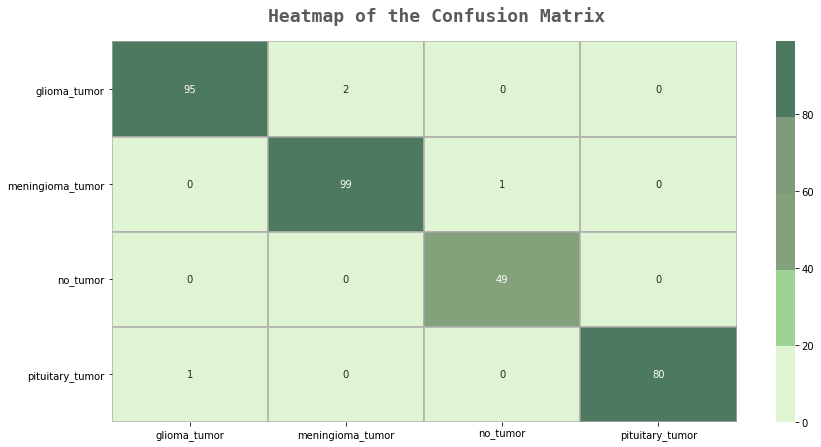
\includegraphics[width=1\textwidth]{conf-matrix-pretrained.png}
	\end{figure}
\end{frame}

	\begin{frame}
		\frametitle{Alcune previsioni}
		\begin{figure}

			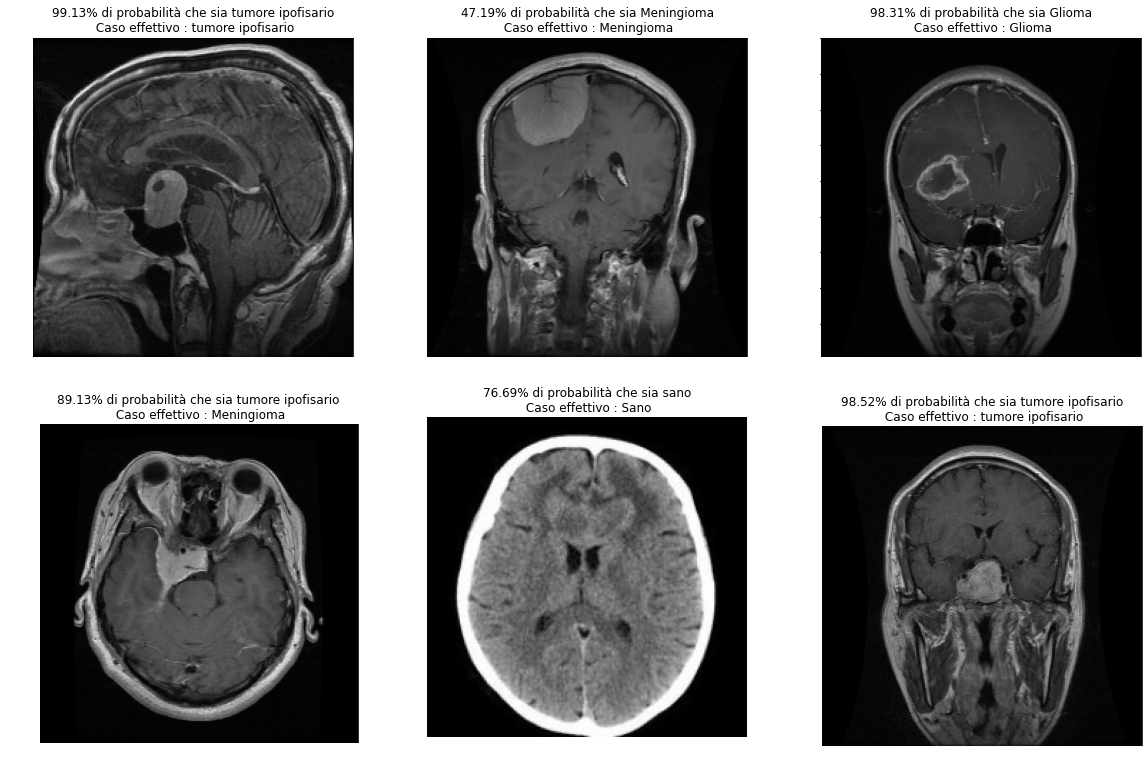
\includegraphics[width=1\textwidth]{results-brain-tumor-alex-net-noise.png}
		\end{figure}
		\end{frame}
	
		\begin{frame}
			\frametitle{ROC e AUC}
			\begin{figure}
				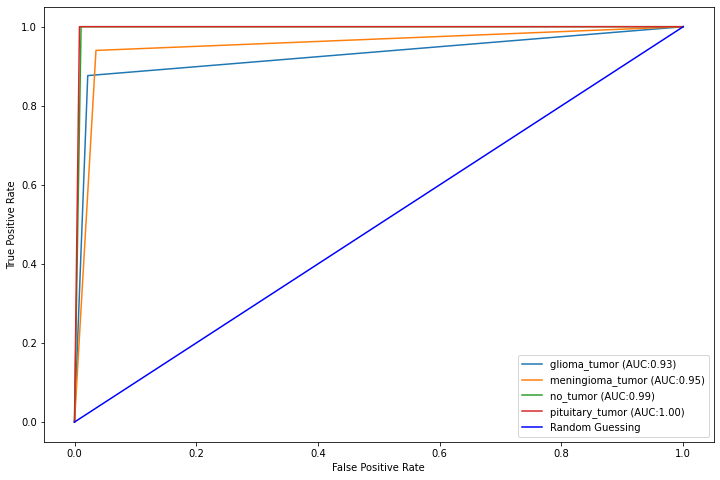
\includegraphics[width=0.5\textwidth]{roc-alexnet.png}
			\end{figure}
			\begin{figure}
				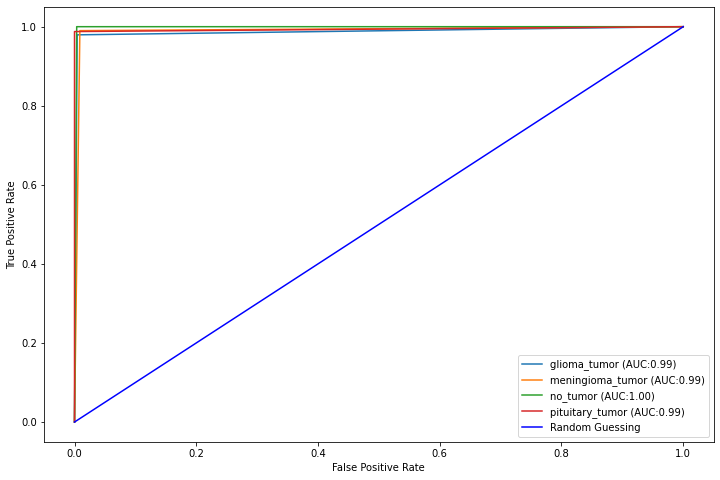
\includegraphics[width=0.5\textwidth]{ROC-pretrained.png}
			\end{figure}
			\end{frame}

			\begin{frame}
				\frametitle{Considerazioni finali}
				In tutti e 3 i casi si sono raggiunti risultati soddisfacenti, nonostante il dataset portasse con sè non poche difficoltà 
				per il suo numero limitato di immagini.\\
				Riassumendo, le tecniche per evitare overfitting in questa esperienza sono state:
				\begin{itemize}
					\item l'uso del Dropout e della Normalizzazione Batch;
					\item l'uso di \emph{jitter} nel set di training;
					\item l'utilizzo del \emph{Transfer learning}.
				\end{itemize}
			\end{frame}

\section{Conclusioni e sviluppi futuri}
\begin{frame}
	\frametitle{Conclusioni e sviluppi futuri}
	Questa esperienza mostra come l'utilizzo delle CNN possa essere esteso a \textbf{vari tipi di classificazione} e che 
	modelli come quelli illustrati possano essere utilizzati per altri tipi di dataset affini. \\
	É sicuramente possibile sfruttare
	i training fatti alle reti neurali sui due dataset, riutilizzarne i pesi per training successivi
	 per l'identificazione di altre patologie visibili da RM o raggi-X, così come possono essere buoni punti di partenza per 
	 la \textbf{segmentazione} di immagini.
	 \begin{figure}
		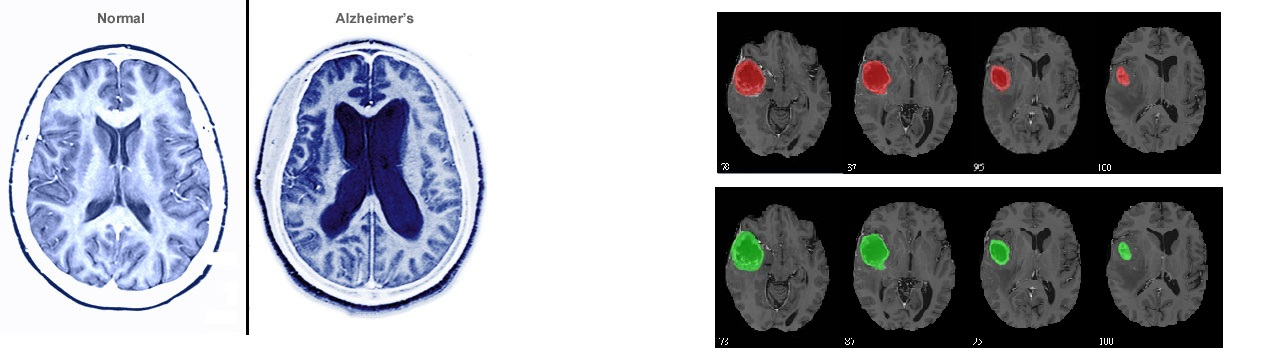
\includegraphics[width=0.9\textwidth]{alzheimer.jpg}
	\end{figure}

\end{frame}

\end{document}